%
% linear.tex
%
% (c) 2020 Prof Dr Andreas Müller, Hochschule Rapperswil
%
\begin{frame}
\frametitle{Lineare Interpolation}
\vspace{-15pt}
\begin{columns}[t]
\begin{column}{0.48\hsize}
\begin{block}{Aufgabe}
Finde eine auf $[x_i,x_{i+1}]$
lineare Funktion
$f(x)$ mit $f(x_i)=f_i$ und $f(x_{i+1})=f_{i+1}$
\end{block}
\uncover<2->{
\begin{block}{Lösung}
	\begin{align*}
		{\color{red}f(x)}
		&\uncover<3->{=\frac{f_{i+1}-f_i}{x_{i+1}-x_i} (x-x_i) + f_i}
		\\
		&\uncover<4->{=\frac{x-x_{i+1}}{x_i-x_{i+1}} f_i}
		\uncover<5->{+\frac{x-x_i}{x_{i+1}-x_i}f_{i+1}}
	\end{align*}
	\vspace{-10pt}
	\begin{align*}
		\uncover<6->{l_i(x)}
		&\uncover<6->{=\frac{x-x_{i+1}}{x_i-x_{i+1}}}
		&\uncover<7->{l_{i+1}(x)}
		&\uncover<7->{=\frac{x-x_i}{x_{i+1}-x_i}}
	\end{align*}
\end{block}}
\end{column}
\begin{column}{0.48\hsize}
\begin{center}
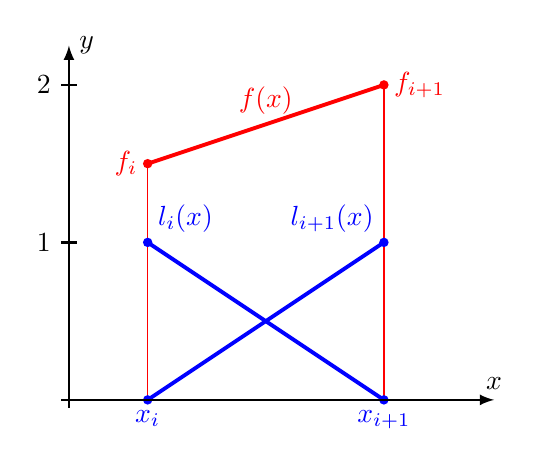
\begin{tikzpicture}[>=latex,thick]

\draw[color=red,line width=0.5pt] (1,0)--(1,3);
\fill[color=red] (1,3) circle[radius=0.06];
\node[color=red] at (1,3) [left] {$f_i$};
\draw[color=red,line width=0.5pt] (4,0)--(4,4);
\fill[color=red] (4,4) circle[radius=0.06];
\node[color=red] at (4,4) [right] {$f_{i+1}$};

\uncover<2->{
	\draw[color=red,line width=1.4pt] (1,3)--(4,4);
	\node[color=red] at (2.5,3.5) [above] {$f(x)$};
}
\uncover<4->{
	\draw[color=blue,line width=1.4pt] (1,2)--(4,0);
	\fill[color=blue] (1,2) circle[radius=0.06];
}
\uncover<6->{
	\node[color=blue] at (1,2) [above right] {$l_i(x)$};
}
\uncover<5->{
	\draw[color=blue,line width=1.4pt] (1,0)--(4,2);
	\fill[color=blue] (4,2) circle[radius=0.06];
}
\uncover<7->{
	\node[color=blue] at (4,2) [above left] {$l_{i+1}(x)$};
}

\fill[color=blue] (1,0) circle[radius=0.06];
\node[color=blue] at (1,0) [below] {$x_i$};
\fill[color=blue] (4,0) circle[radius=0.06];
\node[color=blue] at (4,0) [below] {$x_{i+1}$};

\draw[->] (0,-0.1)--(0,4.5) coordinate[label={right:$y$}];
\draw[->] (-0.1,0)--(5.4,0) coordinate[label={$x$}];
\draw (-0.1,2)--(0.1,2);
\draw (-0.1,4)--(0.1,4);
\node at (-0.1,2) [left] {$1$};
\node at (-0.1,4) [left] {$2$};

\end{tikzpicture}
\end{center}
\vspace{-10pt}
\begin{align*}
\uncover<6->{l_i(x_i)     }&\uncover<6->{= 1}&\uncover<7->{ l_{i+1}(x_i)    }&\uncover<7->{= 0}\\
\uncover<6->{l_i(x_{i+1}) }&\uncover<6->{= 0}&\uncover<7->{ l_{i+1}(x_{i+1})}&\uncover<7->{= 1}
\end{align*}
\end{column}
\end{columns}
\end{frame}
